\begin{problem}
  \begin{figure}[H]
    \centering
    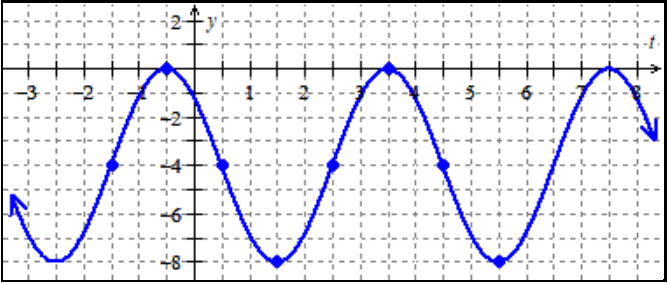
\includegraphics[width=0.8\textwidth]{images/week-3a.png}
    \caption{}
    \label{fig:week_3a}
  \end{figure}

  \begin{itemize}
    \item Use the \textbf{\textit{sine function}} to construct an algebraic rule
      (i.e., a "formula") for the function $f$ graphed in Figure 1. \textbf{[$4$
      points]}
    \item Use the \textbf{\textit{cosine function}} to construct an algebraic
      rule (i.e., a "formula") for the function $f$ graphed in Figure 1.
      \textbf{[$4$ points]}
  \end{itemize}
\end{problem}

\begin{solution}
  \[
  y = A\sin(\omega(t - h)) + k \textrm{ or } y = A\cos(\omega(t - h)) + k
  \].

  Where:
  \begin{center}
    midline: $y = k$ \\
    amplitude:  $\mid A \mid$ \\
    period: $\frac{2\pi}{\mid \omega \mid}$ \\
    horizontal shift: $h$ units \\
    angular frequency: $\omega$ radians per unit of $t$
  \end{center}

  When we look at the graph, we can tell that the midline is $-4$. Also, if
  you want to make sure, you do the following:
  $\frac{f_{\textrm{max}} + f_{\textrm{min}}}{2}$

  To find the amplitude, we look at the midline and count how many units it
  takes to get to either the minimum or maximum. So, our amplitude is $4$.

  To get the period, you can go either maximum to maximum or minimum to
  minimum, which is $4$. Now, we solve for $\omega$.
  \[
  \frac{2\pi}{\omega} = 4 \implies \omega = \frac{\pi}{2}
  \].

  I don't really understand how we would get $h$, but I'm guessing you would
  use $2.5$ for sin and for cos would be $\frac{1}{2}$.

  Here's the final equation:

  \[
  y = 4\sin \left(\frac{\pi}{2}(t - 2.5)\right) - 4 \textrm{ and }
  y = 4\cos \left(\frac{\pi}{2}(t - 0.5)\right) - 4
  \].
\end{solution}

\newpage

\begin{problem}
  \begin{figure}[H]
    \centering
    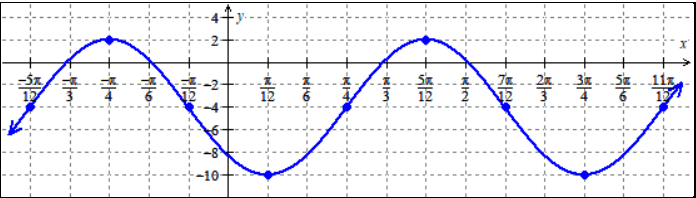
\includegraphics[width=0.8\textwidth]{images/week-3b.png}
    \caption{}
    \label{fig:week_3b}
  \end{figure}

  \begin{itemize}
    \item Use the \textbf{\textit{sine function}} to construct an algebraic rule
      (i.e., a "formula") for the sinusoidal function $g$ graphed in figure 2.
      \textbf{[$4$ points]}
    \item Use the \textbf{\textit{cosine function}} to construct an algebraic
      rule (i.e., a "formula") for the sinusoidal function $g$ graphed in figure
      2. \textbf{[$4$ points]}
  \end{itemize}
\end{problem}

\begin{solution}
  \[
  y = A\sin(\omega(t - h)) + k \textrm{ or } y = A\cos(\omega(t - h)) + k
  \].

  Where:
  \begin{center}
    midline: $y = k$ \\
    amplitude:  $\mid A \mid$ \\
    period: $\frac{2\pi}{\mid \omega \mid}$ \\
    horizontal shift: $h$ units \\
    angular frequency: $\omega$ radians per unit of $t$
  \end{center}

  When we look at the graph, we can tell that the midline is $-4$. Also, if
  you want to make sure, you do the following:
  $\frac{f_{\textrm{max}} + f_{\textrm{min}}}{2}$

  To find the amplitude, we look at the midline and count how many units it
  takes to get to either the minimum or maximum. So, our amplitude is $4$.

  To get the period, you can go either maximum to maximum or minimum to
  minimum, which is $\frac{2\pi}{3}$. Now, we solve for $\omega$.
  \[
  \frac{2\pi}{\omega} = \frac{2\pi}{3} \implies \omega = 3
  \].

  I don't really understand how we would get $h$, but I'm guessing you would
  use $\frac{\pi}{4}$ for sin and for cos would be $\frac{7\pi}{12}$.

  Here's the final equation:

  \[
  y = 4\sin \left(3 \left(t - \frac{\pi}{4}\right)\right) - 4 \textrm{ and }
  y = 4\cos \left(3 \left(t - \frac{7\pi}{12}\right)\right) - 4
  \].
\end{solution}

\newpage

\begin{problem}
  Draw a graph of at least two periods of the function $F(x) = 4\sin
  \left(2x - \frac{\pi}{2}\right) + 2$ by
  \begin{itemize}
    \item plotting the points where the graph intersects the midline
    \item plotting the points where the graph achieves maximum and minimum
      values
    \item connecting these points with an appropriately curved sinusoidal wave.
  \end{itemize}
  Draw an \textbf{accurate} graph and \textbf{label} the scale on the axes.
  \textbf{[$4$ points]}
\end{problem}

\begin{solution}
  \begin{figure}[htpb]
    \centering
    \incfig{week-3}
    \caption{}
    \label{fig:week_3}
  \end{figure}
\end{solution}
